\section{Задание 2. Обзор интерфейса Ubuntu.}

\subsection{Пункт 1}

Представить рабочий стол Ubuntu, объяснить основные элементы интерфейса, таких как панель задач, меню приложений и другие.

\textbf{Ответ:}

Рабочий стол Ubuntu \ref{fig:desktopUbuntu} :

\begin{figure}[!h]
    \centering
    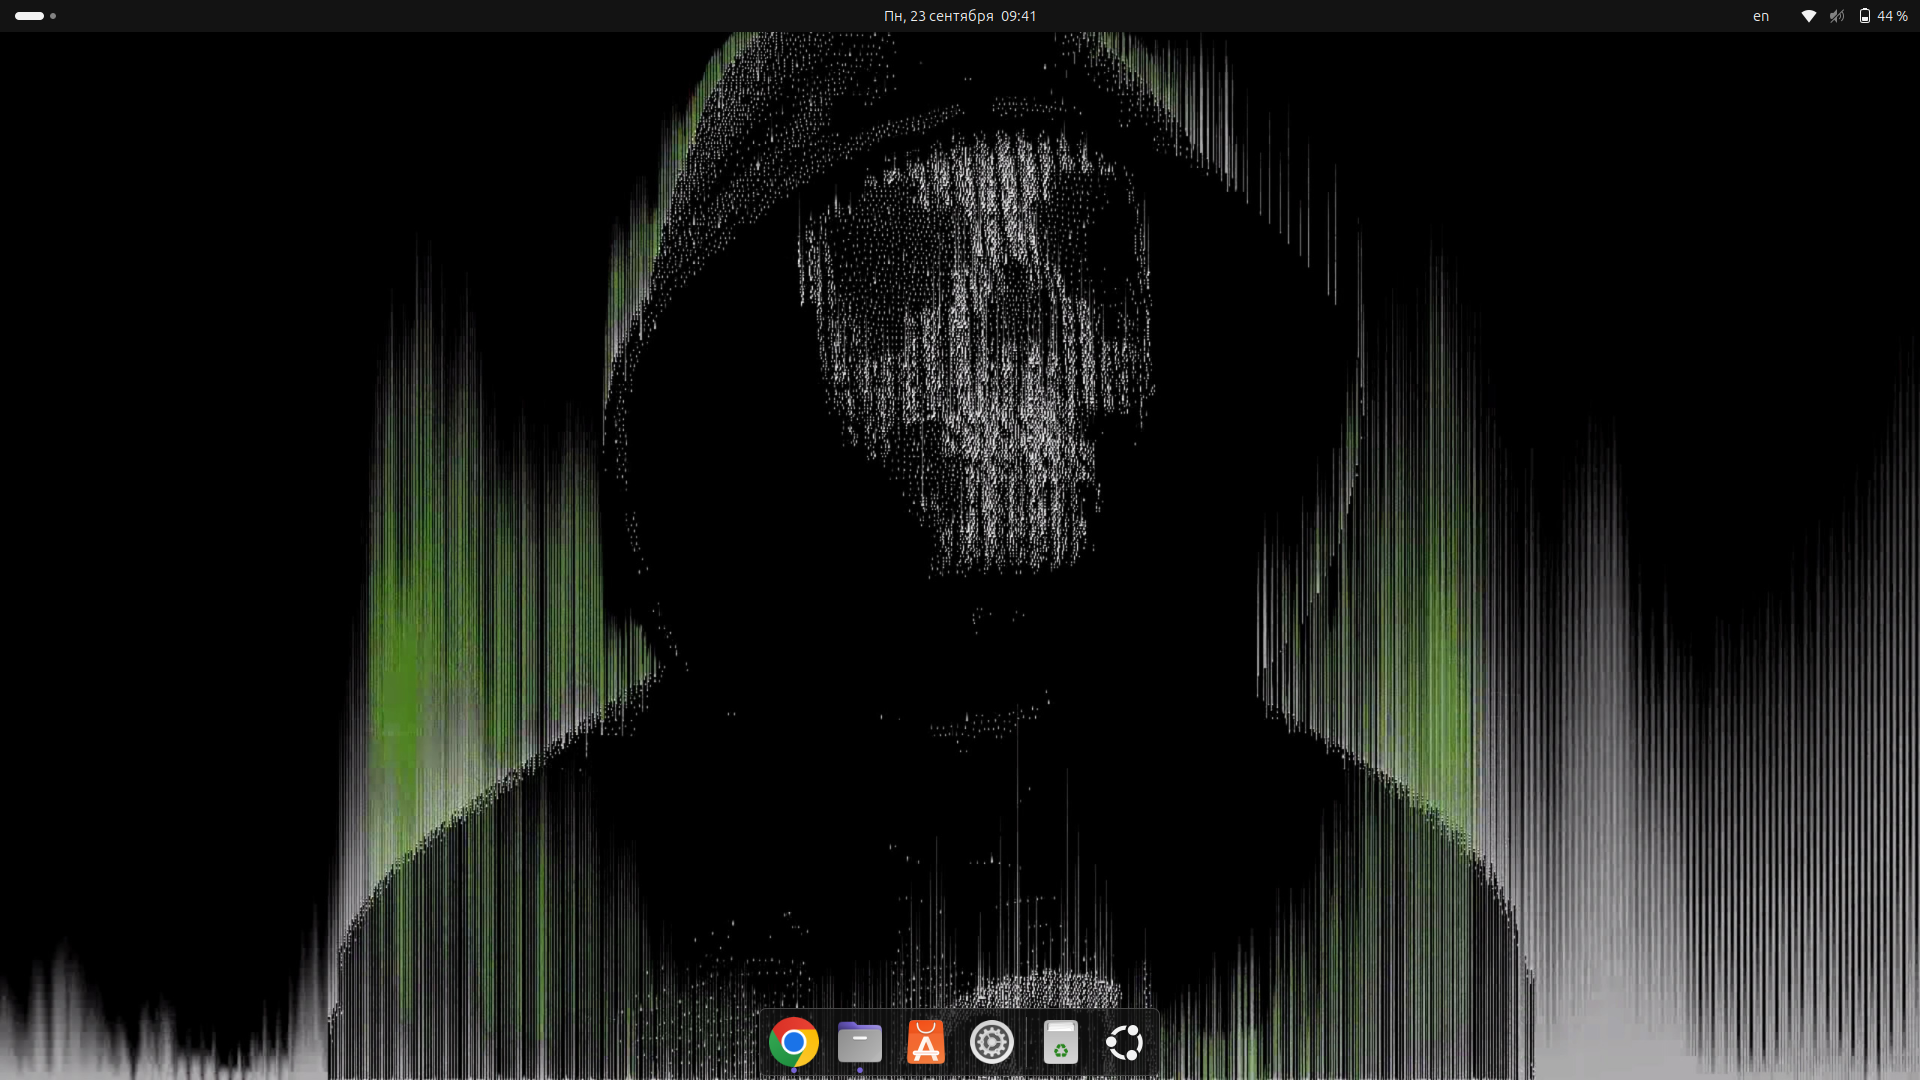
\includegraphics[width = 0.8\textwidth]{images/desktopUbuntu.png}
    
    \caption{Рабочий стол Ubuntu}
    
    \label{fig:desktopUbuntu}
\end{figure}

Панель задач \ref{fig:taskPanel} :

\begin{figure}[!h]
    \centering
    
\includegraphics[width = 0.8\textwidth]{images/taskPanel.png}
    
    \caption{Панель задач}
    
    \label{fig:taskPanel}
\end{figure}

\newpage

Меню приложений \ref{fig:menuApplications} :

\begin{figure}[!h]
    \centering
    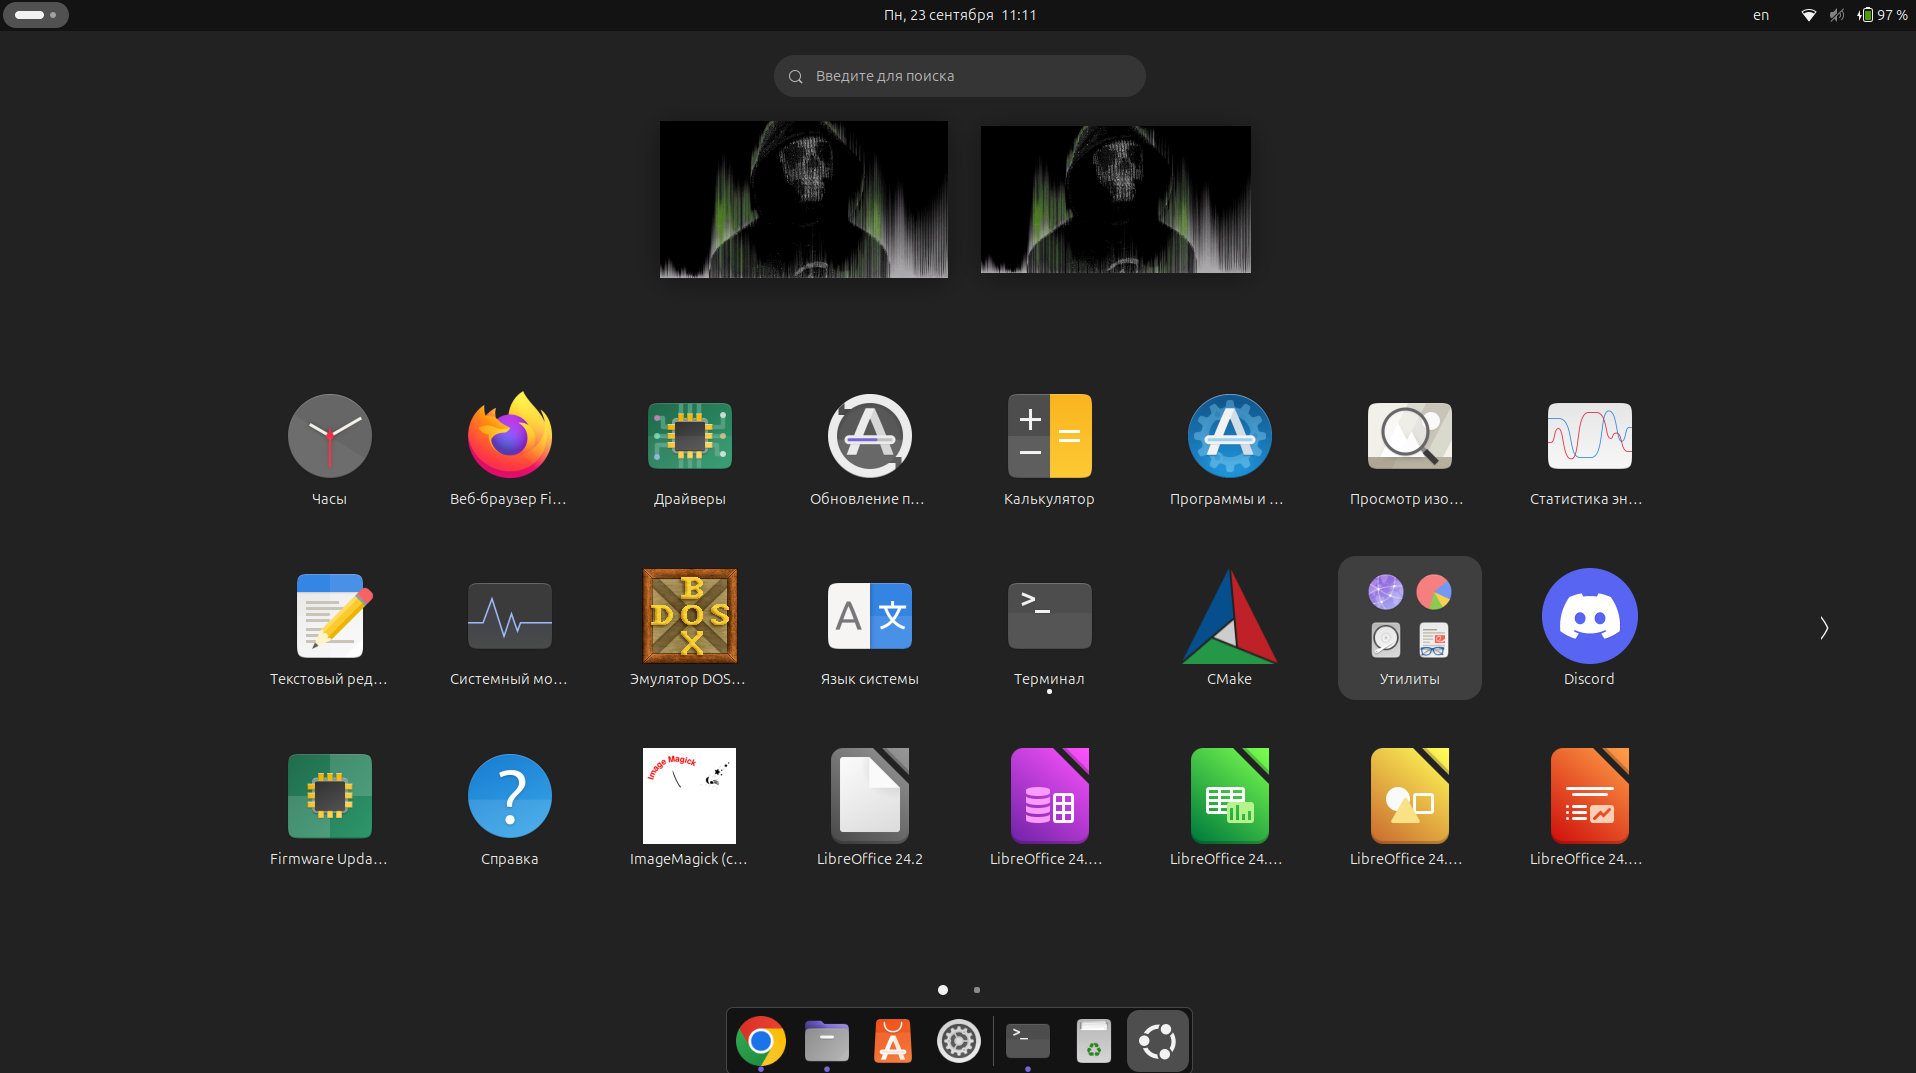
\includegraphics[width = 0.8\textwidth]{images/menuApplications.png}
    
    \caption{Меню приложений}
    
    \label{fig:menuApplications}
\end{figure}

Системное меню \ref{fig:menuSystem} :

\begin{figure}[!h]
    \centering
    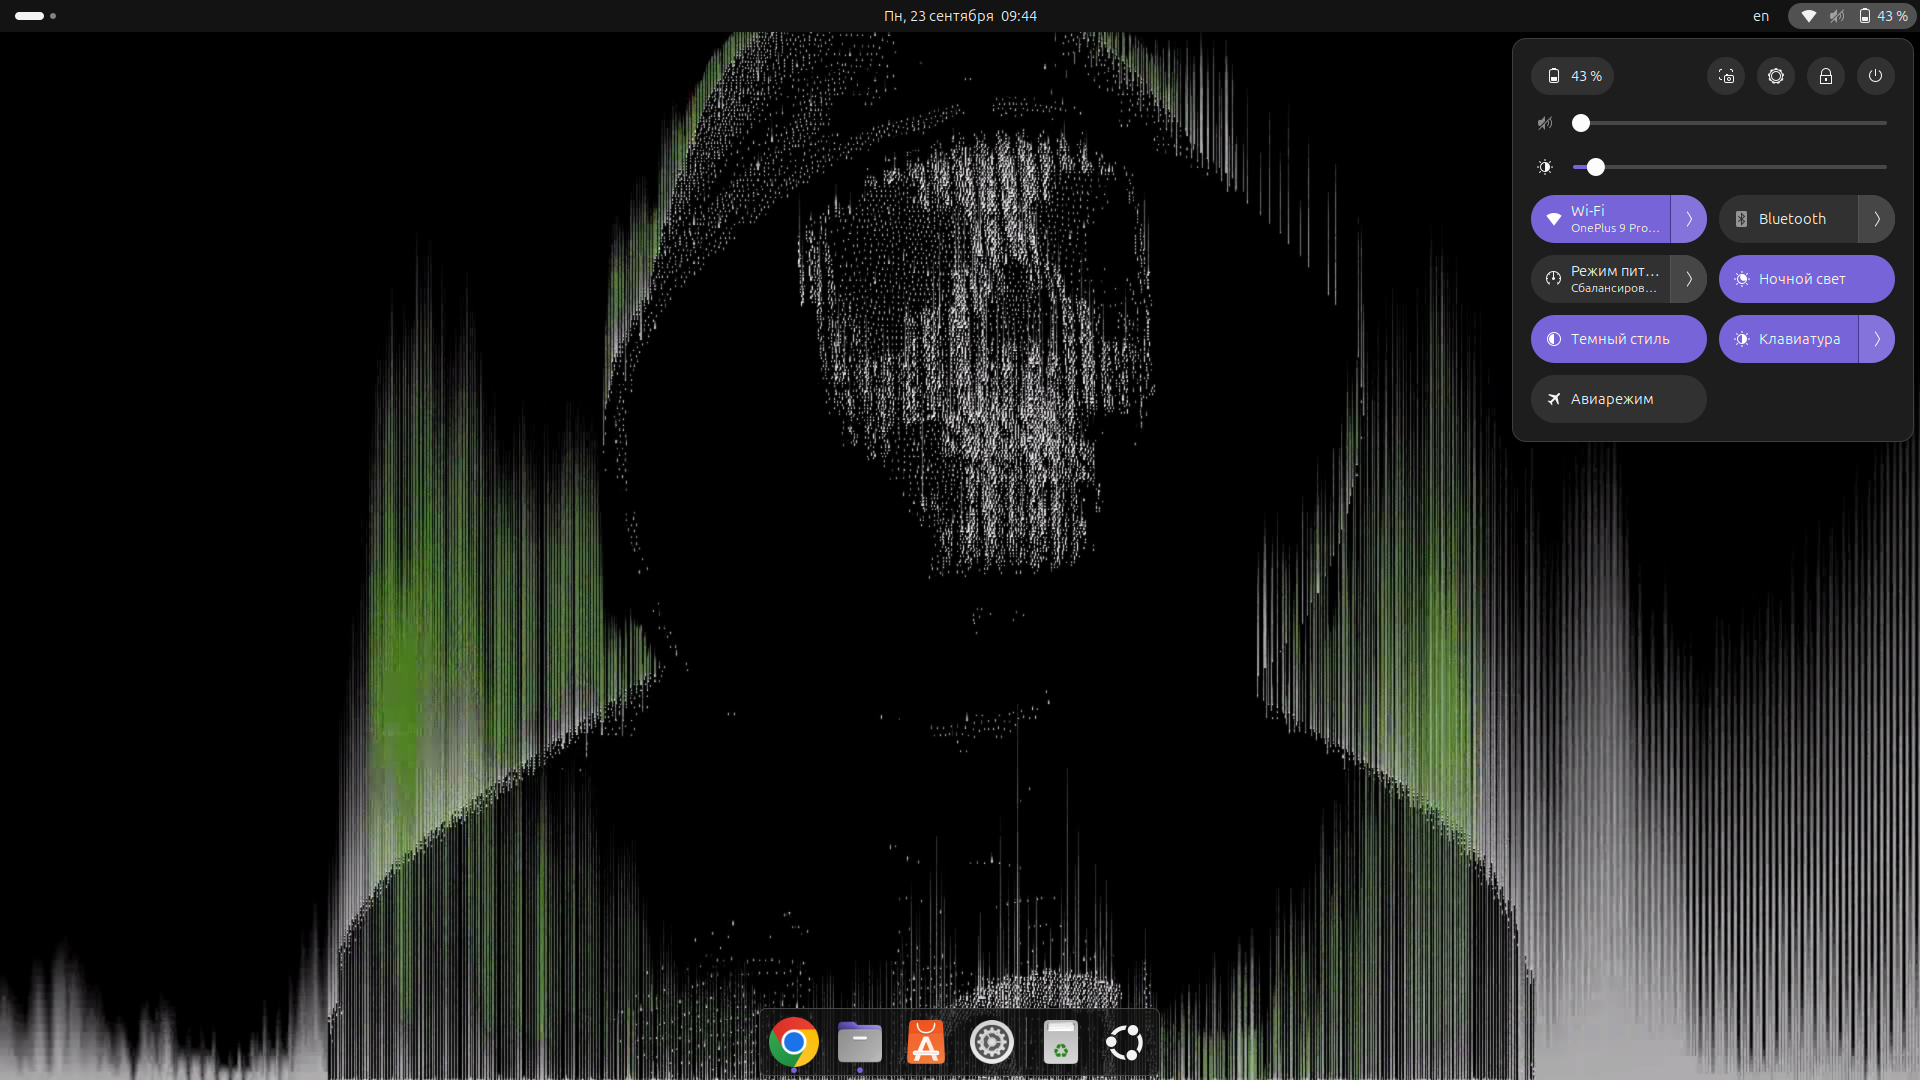
\includegraphics[width = 0.8\textwidth]{images/menuSystem.png}
    
    \caption{Системное меню}
    
    \label{fig:menuSystem}
\end{figure}

\newpage

Часы, календарь, события \ref{fig:desktopUbuntuCalendar} :

\begin{figure}[!h]
    \centering
    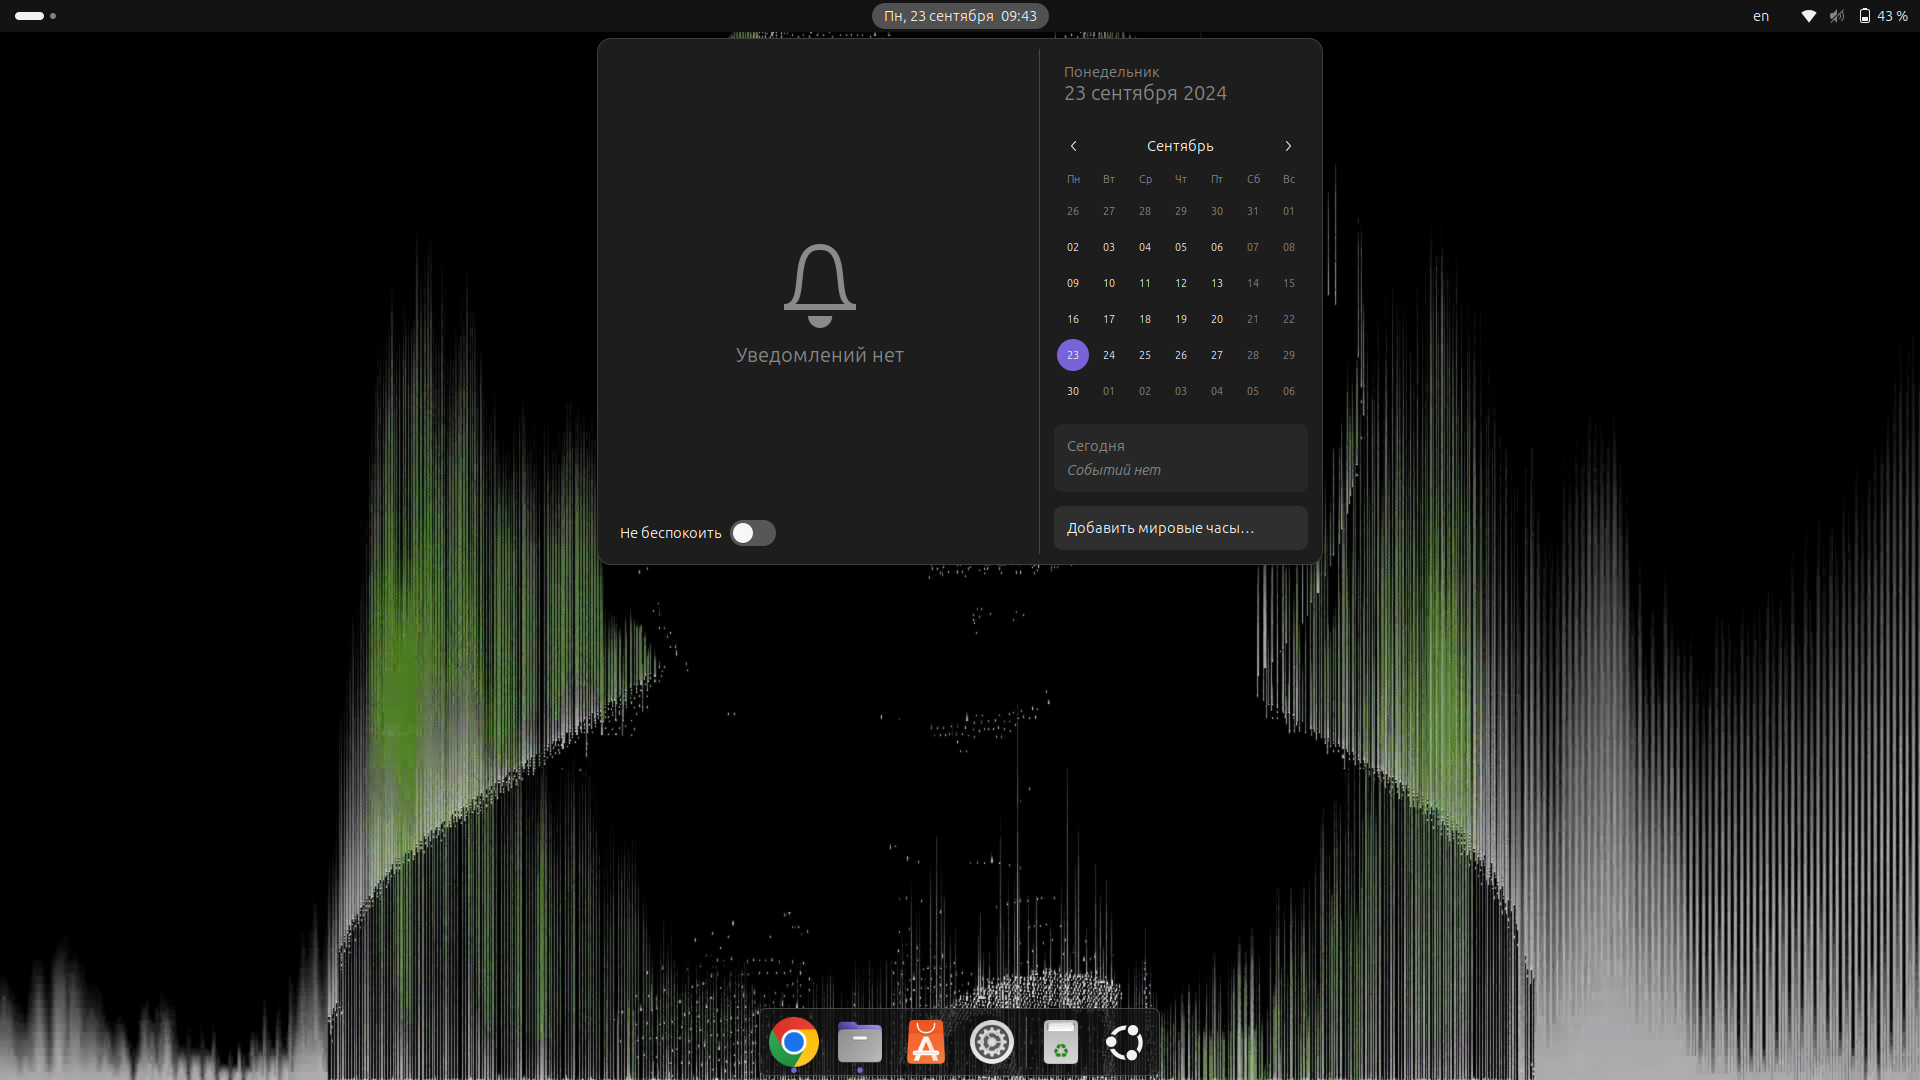
\includegraphics[width = 0.8\textwidth]{images/desktopUbuntuCalendar.png}
    
    \caption{Часы, календарь, события}
    
    \label{fig:desktopUbuntuCalendar}
\end{figure}

\subsection{Пункт 2}

Показать, как открыть и управлять приложениями ОС, как открыть и управлять окнами на рабочем столе.


Открыть системное приложение \ref{fig:openApp} :

\begin{figure}[!h]
    \centering
    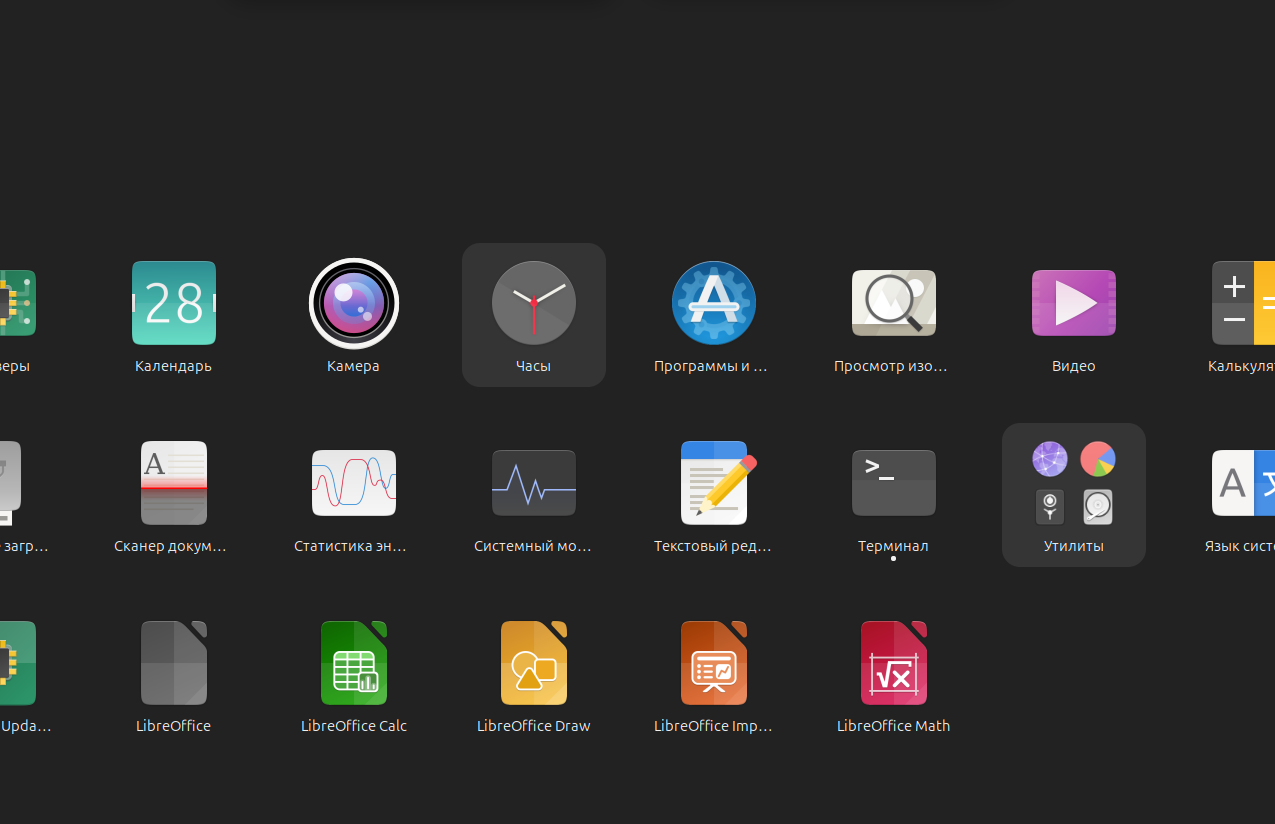
\includegraphics[width = 0.8\textwidth]{images/openApp.png}
    
    \caption{Открыть системное приложение}
    
    \label{fig:openApp}
\end{figure}

\newpage

Закрыть системное приложение \ref{fig:closeApp} :

\begin{figure}[!h]
    \centering
    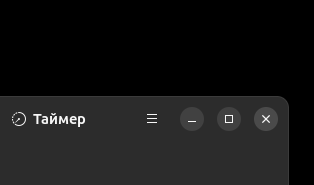
\includegraphics[width = 0.8\textwidth]{images/closeApp.png}
    
    \caption{Закрыть системное приложение}
    
    \label{fig:closeApp}
\end{figure}

Открыть приложение \ref{fig:openAppDesktop} :

\begin{figure}[!h]
    \centering
    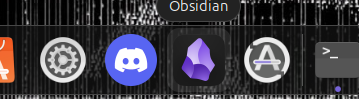
\includegraphics[width = 0.8\textwidth]{images/openAppDesktop.png}
    
    \caption{Системное меню}
    
    \label{fig:openAppDesktop}
\end{figure}

\newpage

Закрыть приложение \ref{fig:closeAppDesktop} :

\begin{figure}[!h]
    \centering
    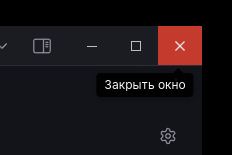
\includegraphics[width = 0.8\textwidth]{images/closeAppDesktop.png}
    
    \caption{Закрыть приложение}
    
    \label{fig:closeAppDesktop}
\end{figure}

Свернуть приложение \ref{fig:roll} :

\begin{figure}[!h]
    \centering
    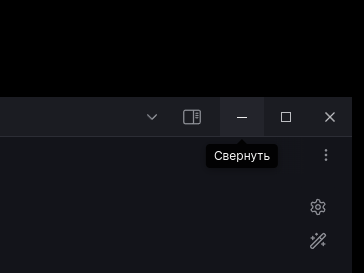
\includegraphics[width = 0.8\textwidth]{images/roll.png}
    
    \caption{Свернуть приложение}
    
    \label{fig:roll}
\end{figure}


Развернуть приложение \ref{fig:unroll} :

\begin{figure}[!h]
    \centering
    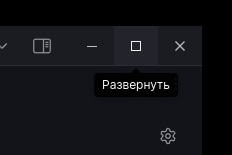
\includegraphics[width = 0.8\textwidth]{images/unroll.png}
    
    \caption{Развернуть приложение}
    
    \label{fig:unroll}
\end{figure}

\subsection{Пункт 3}

Настроить и персонализировать интерфейс Ubuntu

Настройка панели задач \ref{fig:settingUbuntu1} :

\begin{figure}[!h]
    \centering
    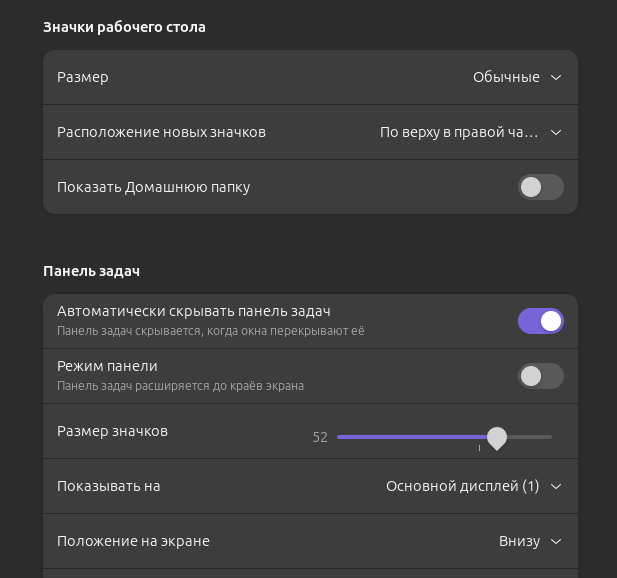
\includegraphics[width = 0.7\textwidth]{images/settingUbuntu1.png}
    
    \caption{Настройка панели задач}
    
    \label{fig:settingUbuntu1}
\end{figure}

\newpage

Настройка темы, обоев и тд \ref{fig:settingUbuntu2} :

\begin{figure}[!h]
    \centering
    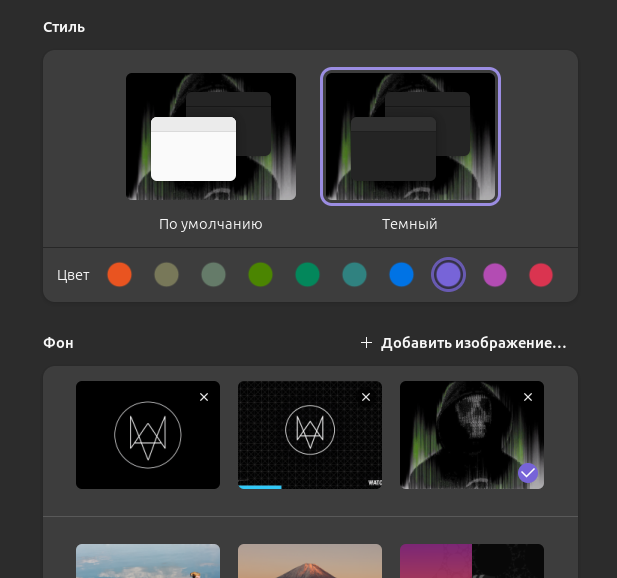
\includegraphics[width = 0.8\textwidth]{images/settingUbuntu2.png}
    
    \caption{Настройка темы, обоев и тд}
    
    \label{fig:settingUbuntu2}
\end{figure}

